\documentclass{VUMIFPSkursinis}
\usepackage{algorithmicx}
\usepackage{algorithm}
\usepackage{algpseudocode}
\usepackage{amsfonts}
\usepackage{amsmath}
\usepackage{bm}
\usepackage{caption}
\usepackage{color}
\usepackage{float}
\usepackage{graphicx}
\usepackage{listings}
\usepackage{subfig}
\usepackage{wrapfig}

\usepackage{enumitem}
%PAKEISTA, tarpai tarp sąrašo elementų
\setitemize{noitemsep,topsep=0pt,parsep=0pt,partopsep=0pt}
\setenumerate{noitemsep,topsep=0pt,parsep=0pt,partopsep=0pt}

% Titulinio aprašas
\university{Vilniaus universitetas}
\faculty{Matematikos ir informatikos fakultetas}
\department{Programų sistemų katedra}
\papertype{Programų kūrimo proceso laboratorinis darbas}
\title{Žaidimų pristatymų įmonės informacinės sistemaos}
\titleineng{Description of the development process of the "Another One" company}
\status{4 kurso studentai}
\author{Nedas Valentinovičius, Linas Valiukonis}
\supervisor{Audronė Lupeikienė, M. Darbuot., Dr.}
\date{Vilnius – \the\year}

% Nustatymai
%\setmainfont{Palemonas}
% \bibliography{bibliografija}

\begin{document}
	
\maketitle
\cleardoublepage\pagenumbering{arabic}
\setcounter{page}{2}

\sectionnonum{Anotacija}
Komandos nariai ir jų kontaktiniai duomenys:
\begin{itemize}
	\item Linas Valiukonis, paštas: linas.valiukonis@mif.stud.vu.lt
	\item Nedas Valentinoviičus, paštas: nedas.valentinovičius@mif.stud.vu.lt
\end{itemize}

\tableofcontents

\sectionnonum{Įvadas}
DUDE I DO NOT GIVE A SINGLE FLYING FUCK ABOUT THIS

\section{Panaudotų dokumentų sąrašas}

%\begin{figure}[H]
%    \centering
%    \includegraphics[scale=0.8]{img/Procesudiagrama}
%    \caption{Kūrimo procesų diagrama}
%    \label{img:mlp}
%\end{figure}


\newpage
\section{Kompiuterizuojamo objekto anazilė}

\newpage
\subsection{Kompiuterizuojamo verslo objekto apibūdinimas}
Žaidimų pristatymo įmonės verslo sistema pristato klientų įgytas prekias jiems fizižkai ar virtualiai. Paslaugos yra reklamuojamos internetinėje įmonės svetainėje. Sudaromos sutartys su kitomis įmonėmis, kurios nori pasinaudoti mūsų sistema ir išplatinti jų produktus.
\begin{itemize}
	\item Verlslo objektai: produktai (žaidimai, žaidimų konsolės, įranga ir kt.), klientai, pinigai, banko kortelės.
	\item Verslo transakcijos: Apmokėjimas už produktą, produkto pristatymas klientui, produktų pirkimas.
	\item Verslo funkcijos: produktų pirkimų tvarkymas, sutarčių sudarymas, produktų duomenų tvarkymas, klientų duomenų tvarkymas, mokėjimų duomenų tvarkymas, produktų katalogo tvarkymas.
	\item Organizacijos atmintis: produktų registravimo knyga, klientų registravimo knyga, sutarčių registravimo knyga, įvykdytų transakcijų knyga, produktų katalogas.
	\item Verslo aktoriai: įmonės atstovas, vadybininkas ir administratorius.
\end{itemize}
\newpage
\subsection{IS konteksto diagrama. IS išoriniai informacijos srautai}
\begin{figure}[H]
    \centering
    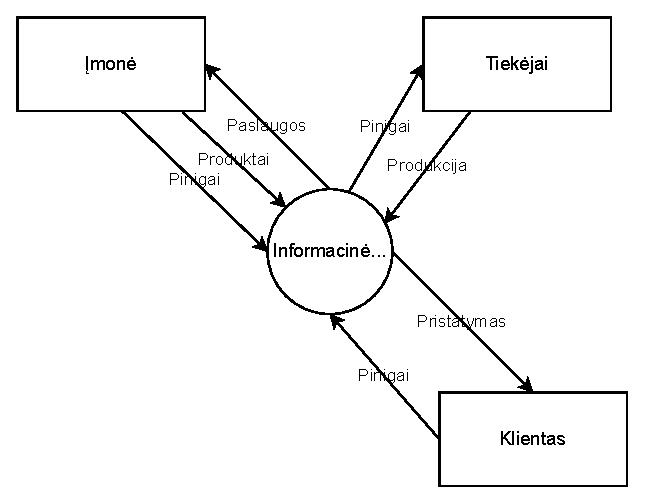
\includegraphics[scale=1]{img/KontekstoDiagrama}
    \caption{Konteksto diagrama}
    \label{img:mlp}
\end{figure}
\newpage
\subsection{IS galimybių medis}

\newpage
\subsection{IS užduotys}

\newpage
\subsection{Informacijos apdorojimo procesai}

\newpage
\subsection{IS saugoma informacija (saugyklos)}

\newpage
\subsection{IS vartotojai ir jų darbo vietos}

\newpage
\subsection{IS inžinieriaus požiūris. Užpildoma antra 1 lentelės eilutė}

\newpage
\subsection{Sudaromas IS posistemių sąrašas ir nurodomi jų tipai}

\newpage
\subsection{IS registrų sistema}

\newpage
\section{Pastabos apie dokumentą DĖL VALSTYBĖS INFORMACINIŲ SISTEMŲ GYVAVIMO CIKLO VALDYMO METODIKOS PATVIRTINIMO}

\newpage

\section{Išvados}

\newpage
\sectionnonum{Terminų žodynėlis}
\begin{itemize}
	\item{Trikdžiai -- veikla ar procesus stabdantys veiksniai}
\end{itemize}

\section{Priedai}

\newpage
\section{Pavyzdiniai latexo dalykai, nes dažnai pamirštu}
Citavimo pavyzdžiai: cituojamas vienas šaltinis \cite{PvzStraipsnLt}; cituojami
keli šaltiniai \cite{PvzStraipsnEn, PvzKonfLt, PvzKonfEn, PvzKnygLt, PvzKnygEn,
PvzElPubLt, PvzElPubEn, PvzMagistrLt, PvzPhdEn}.

\begin{enumerate}
	\item Pirmas elementas
	\item Antras elementas
\end{enumerate}

\begin{figure}[H]
    \centering
    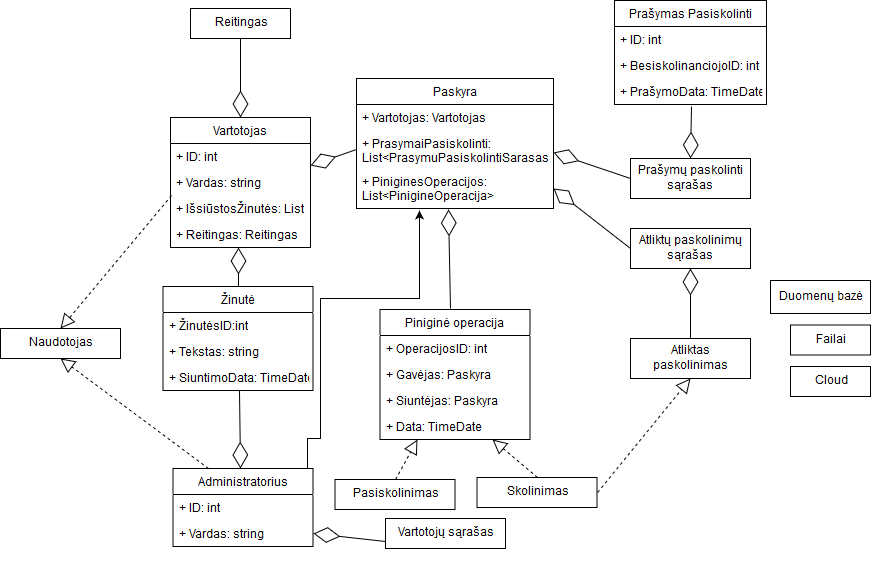
\includegraphics[scale=0.5]{img/DomainModel}
    \caption{Paveikslėlio pavyzdys}
    \label{img:mlp}
\end{figure}

% tablesgenerator.com - converts calculators (e.g. excel) tables to LaTeX
\begin{table}[H]\footnotesize
  \centering
  \caption{Lentelės pavyzdys}
  {\begin{tabular}{|l|c|c|} \hline
    Algoritmas & $\bar{x}$ & $\sigma^{2}$ \\
    \hline
    Algoritmas A  & 1.6335    & 0.5584       \\
    Algoritmas B  & 1.7395    & 0.5647       \\
    \hline
  \end{tabular}}
  \label{tab:table example}
\end{table}

\end{document}